\documentclass[11pt,a4paper]{article}

% ---------------------------------------------------------------------------
% Assignment 1 report - Big Data (ULPGC, 2026-2027)
% Compile with pdflatex (Overleaf: upload this folder including figures/).
% All numbers come from results/raw/benchmark_20261014_222025.csv via
% scripts/analyze.py (tables in results/tables/).
% ---------------------------------------------------------------------------

\usepackage[utf8]{inputenc}
\usepackage[T1]{fontenc}
\IfFileExists{lmodern.sty}{\usepackage{lmodern}\usepackage{microtype}}{}
\usepackage[margin=2.3cm]{geometry}
\usepackage{amsmath,amssymb}
\usepackage{graphicx}
\usepackage{booktabs}
\usepackage{multirow}
\usepackage{xcolor}
\usepackage{listings}
\usepackage{caption}
\usepackage{tabularx}
\usepackage{xurl}
\usepackage[hidelinks]{hyperref}
\emergencystretch=2.5em

\graphicspath{{figures/}{../figures/}}

\lstset{basicstyle=\ttfamily\small, columns=fullflexible, frame=single,
        framerule=0.3pt, rulecolor=\color{gray}, aboveskip=6pt, belowskip=6pt}

\captionsetup{font=small, labelfont=bf}

\newcommand{\repo}{\url{https://github.com/JaviMRO/bigdata-matrix-multiplication}}

\title{\textbf{Assignment 1: Runtime and Memory of Basic Triple-Loop\\
Matrix Multiplication in Python, Java and C}}
\author{Javier Martín Rodríguez\\[2pt]
\small Big Data -- Grado en Ciencia e Ingeniería de Datos, Universidad de Las Palmas de Gran Canaria\\
\small Individual Assignment 1 \quad·\quad Academic year 2026--2027}
\date{15 October 2026}

\begin{document}
\maketitle

\begin{abstract}
\noindent
This study asks how the matrix size $n$ affects the runtime and memory use of the textbook
$O(n^3)$ i-j-k matrix multiplication implemented in Python (CPython 3.12), Java (HotSpot 25)
and C (gcc 16.1, \texttt{-O2}) on one Windows 11 laptop with an Intel Core Ultra~9 275HX.
All three implementations read the same binary input files, use IEEE-754 doubles and the same
loop order, and were validated against NumPy before benchmarking. The multiplication kernel
was timed with monotonic timers for $n = 64$ to $2048$ (5--10 measured repetitions per
configuration, pinned to one performance core), and the peak working set of each process was recorded.
C and Java finished every size up to $n = 2048$; CPython finished up to $n = 1024$
(62.7\,s median) and exceeded the declared 600\,s budget at $n = 2048$. Up to $n = 512$, CPython was
51--187 times slower than C, while Java was 1.1--2.3 times slower. For $n \ge 1024$ C and Java took
almost the same time (Java/C ratio 0.96 and 1.09). Fitted log-log slopes for $n \ge 256$ were above
the algorithmic value of 3 (3.79 C, 3.74 Java, 3.28 Python), mainly because the time per inner-loop
iteration rose sharply between $n = 512$ and $n = 1024$. This is consistent with matrix $B$, accessed
column-wise, no longer fitting in the core's 3\,MB L2 cache. Peak memory approached the
theoretical $24n^2$ bytes for C, was dominated by a $\approx$45\,MB runtime baseline for Java at small
$n$, and was about 5.6 times the raw data size for CPython at $n = 1024$. These conclusions are
limited to the tested implementations, settings, inputs and machine.
\end{abstract}

% ===========================================================================
\section{Introduction and objective}

Dense matrix multiplication is a basic building block of scientific computing and data
processing. Its textbook form performs $n^3$ multiply-add operations for two $n\times n$ matrices,
so runtime is expected to grow cubically with the matrix size. In practice, the measured time also
depends on how a language runtime executes the loops and on how the data moves through the memory
hierarchy. This first assignment sets up a validated, reproducible baseline that later
assignments (optimisation, sparse, parallel and distributed multiplication) will reuse.

\paragraph{Research question.}
\emph{How does the matrix size $n$ affect the runtime and memory use of the basic triple-loop dense
matrix multiplication implemented in Python, Java and C, on one fixed Windows laptop?}

The factor varied is $n$ (side of a square matrix); the language implementation is the second
factor. The outcomes are the kernel execution time and the peak memory of the process.

\paragraph{Hypotheses (predictions, stated before measuring).}
\begin{enumerate}
  \item[H1] Runtime grows approximately as $n^3$ in all three implementations; the log-log slope may
        exceed 3 once matrices no longer fit in cache, because the i-j-k order reads $B$ by columns.
  \item[H2] C is fastest, Java is close to C after JIT warm-up, and CPython is one to two orders of
        magnitude slower.
  \item[H3] Peak process memory is dominated by runtime overhead at small $n$ and by matrix storage at
        large $n$. CPython uses much more memory per element than C and Java (8 bytes per double).
\end{enumerate}

% ===========================================================================
\section{Background}

\paragraph{Algorithm.} For $C = AB$ with $A, B \in \mathbb{R}^{n\times n}$, the definition
$c_{ij} = \sum_{k=1}^{n} a_{ik} b_{kj}$ leads directly to three nested loops
(i-j-k order) with $n^3$ multiply-adds and $\Theta(n^2)$ storage~\cite{golub2013}. In
row-major storage, the innermost loop reads a row of $A$ contiguously but reads a column of $B$
with a stride of $n$ elements ($8n$ bytes). Once $B$ no longer fits in a cache level,
almost every access to $B$ misses that level. Cache behaviour, rather than arithmetic, then limits
performance~\cite{drepper2007,hennessy2017}. When the stride is a large power of two, consecutive
accesses also map to the same cache sets, which causes additional conflict
misses~\cite{lam1991}.

\paragraph{Execution models.} C is compiled ahead of time to native code. Java is compiled to
bytecode that HotSpot first interprets and then compiles to native code with its tiered JIT
compilers, so the first executions are slower and warm-up runs are needed~\cite{georges2007}.
CPython interprets bytecode. Each \texttt{float} is a separate heap object, and each element
access goes through dynamic type dispatch and reference counting, so the cost per operation is much
higher.

\paragraph{Floating-point accuracy.} Different summation orders give slightly different results.
For an inner product of length $n$ computed in floating point, the forward error satisfies
$|\hat{c}_{ij} - c_{ij}| \le \gamma_n \sum_k |a_{ik}||b_{kj}|$ with
$\gamma_n = nu/(1-nu)$ and unit roundoff $u = 2^{-53}$~\cite{higham2002}. This bound is the basis of
the correctness tolerance (Section~\ref{sec:validation}).

% ===========================================================================
\section{Methodology}

\subsection{Implementations}
All three kernels implement the same i-j-k loop with a local accumulator. No library matrix
multiplication, blocking, loop reordering, threads or explicit SIMD are used.

\begin{lstlisting}
for i in 0..n-1:
    for j in 0..n-1:
        sum = 0.0
        for k in 0..n-1:
            sum += A[i][k] * B[k][j]
        C[i][j] = sum
\end{lstlisting}

\begin{itemize}
  \item \textbf{C} (\texttt{src/c/matmul.c}): one contiguous \texttt{malloc}'d \texttt{double}
        array per matrix, row-major, element $(i,j)$ at \texttt{i*n+j}. Compiled with
        \texttt{gcc -O2 -std=c17 -Wall -Wextra} (no \texttt{-march=native}, no \texttt{-ffast-math}).
  \item \textbf{Java} (\texttt{src/java/MatMul.java}): one \texttt{double[]} per matrix with the same
        row-major indexing as C. Compiled with default \texttt{javac}; run as
        \texttt{java -Xmx4g -cp build MatMul} (default G1 collector, tiered JIT).
  \item \textbf{Python} (\texttt{src/python/matmul.py}): list of lists of \texttt{float}, the
        idiomatic CPython representation. Each element is an 8-byte pointer to a 24-byte
        \texttt{float} object, so the storage layout necessarily differs from C and Java. NumPy is not
        used in the kernel.
\end{itemize}

Each program reads $A$ and $B$ from file, allocates $C$ once, runs $W$ warm-up and $R$ measured
repetitions in the same process, and prints one CSV line per repetition (time in nanoseconds and
a checksum, the row-major sum of $C$). The checksum is computed outside the timed region and
printed, so the result is always consumed. In C, Java and Python the checksum loop adds the
elements in the same order.

\subsection{Inputs}
NumPy~2.2.6 generated the inputs once with \texttt{numpy.random.default\_rng(seed)} (PCG64), drawing
values uniformly in $[-1, 1)$ as float64. $A$ uses seed 20261016 and $B$ seed 20261017,
with a fresh generator for every $n$. The matrices are stored as raw little-endian float64 files in
row-major order, without a header, so every implementation reads exactly the same logical
inputs. \texttt{data/manifest.json} records the seeds, the SHA-256 hash of every file and the NumPy reference
checksum of $AB$. The \texttt{.bin} files are not committed because
\texttt{generate\_inputs.py} regenerates them bit for bit.

\subsection{Environment}
Table~\ref{tab:env} summarises the environment, as collected automatically by
\texttt{scripts/system\_info.py} (\texttt{results/system\_info.json}).

\begin{table}[htbp]
  \centering\small
  \caption{Hardware and software environment (fixed for all runs).}
  \label{tab:env}
  \begin{tabularx}{\linewidth}{lX}
    \toprule
    CPU & Intel Core Ultra 9 275HX, hybrid: 8 P-cores + 16 E-cores, 24 logical CPUs (no SMT) \\
    Caches (P-core) & L1d 48\,KB, L2 3\,MB per core, L3 36\,MB shared \\
    RAM & 31.4\,GiB \\
    OS & Windows 11 Home (Core) 25H2, build 26200.9711 \\
    Power & AC power, Windows power mode ``Best performance'' \\
    C & gcc 16.1.0 (MinGW-W64 x86\_64-ucrt-posix-seh), \texttt{-O2 -std=c17} \\
    Java & Eclipse Temurin OpenJDK 25.0.4.1 LTS (HotSpot, G1 GC), \texttt{-Xmx4g} \\
    Python & CPython 3.12.10 (64-bit, MSC build) \\
    Analysis & NumPy 2.2.6, pandas 3.0.0, matplotlib 3.10.8, psutil 7.2.2, SciPy \\
    \bottomrule
  \end{tabularx}
\end{table}

\paragraph{Process control.} The orchestrator \texttt{scripts/run\_benchmarks.py} starts each
(language, $n$) configuration as a fresh process with \texttt{HIGH\_PRIORITY\_CLASS}. It pins the process
to a single P-core logical CPU (CPU 23), chosen with \texttt{GetSystemCpuSetInformation} as one of the
CPUs with the highest efficiency class~\cite{ms_cpuset}, so that the hybrid scheduler cannot move it to
an E-core. The C and Python kernels are single-threaded. The JVM additionally runs JIT-compiler
and GC threads, and the process affinity confines all of them to the same CPU. The orchestrator
checks AC power, the power mode and that validation passed before it starts. During the run only
Visual Studio Code was open, the benchmark was launched from its integrated terminal, and the laptop
stood on a desk (\texttt{results/run\_notes.md}).

\subsection{Measurement protocol}
\begin{itemize}
  \item \textbf{Timing boundary:} kernel only. Input reading, allocation and initialisation of $C$,
        and the checksum are outside the timed region.
  \item \textbf{Timers:} monotonic, in nanoseconds: \texttt{QueryPerformanceCounter} in C~\cite{ms_qpc},
        \texttt{System.nanoTime()} in Java and \texttt{time.perf\_counter\_ns()} in Python.
  \item \textbf{Sizes:} $n \in \{64, 128, 256, 512, 1024, 2048\}$. Python at $n = 2048$ was attempted
        once (no warm-up) to document the limit.
  \item \textbf{Repetitions:} 10 measured for $n \le 256$ and 5 for $n \ge 512$. Warm-ups are the same for all
        languages: 2 for $n \le 512$ and 1 for $n \ge 1024$. Warm-ups are kept in the raw CSV and
        excluded from statistics.
  \item \textbf{Order:} ascending $n$, with the order of languages rotated within each $n$ to avoid a
        systematic thermal bias, and a 5\,s pause between processes.
  \item \textbf{Budgets (declared before running):} at most 600\,s per single multiplication (the
        process is killed if no new result line arrives within 600\,s and the run is recorded as a timeout).
        The peak working set may not exceed 50\% of physical RAM (16.8\,GB).
  \item \textbf{Memory metric:} \emph{peak working set} of the whole process
        (\texttt{PeakWorkingSetSize} from \texttt{GetProcessMemoryInfo}~\cite{ms_pmc}), read by the
        orchestrator on the process handle after exit. This single tool is used for all three languages.
        For comparison we also report the theoretical storage of three dense matrices, $3\cdot 8n^2$ bytes.
        The peak working set includes the runtime itself (JVM, interpreter, C runtime) and any temporary
        buffers, so it is a process-level measure and not an array-size measure.
  \item \textbf{Statistics:} median with first and third quartiles (IQR); per-iteration time
        $t/n^3$; and a least-squares fit of $\log t = a + b\log n$ on all measured repetitions with
        $n \ge 256$, with a 95\% confidence interval for the slope $b$ (\texttt{scripts/analyze.py}).
\end{itemize}

\subsection{Correctness checks}\label{sec:validation}
\texttt{scripts/validate.py} runs every implementation through its normal command line with a
\texttt{--dump} option and compares the dumped $C$ with the expected result. The test cases are:
identity on the left and on the right and the zero matrix ($n = 33$, exact); hand-checked
$2\times2$ and $3\times3$ integer-valued cases (exact); random matrices for
$n \in \{1, 2, 7, 33, 64, 128, 256\}$ against \texttt{numpy.matmul}; and every benchmark input
($n = 64$ to $2048$; Python up to 1024). For non-exact cases an element passes if
$|C - C_{\text{ref}}| \le 2\gamma_n(|A|\,|B|)$ element-wise. The factor 2 covers the rounding errors
of both the tested result and the NumPy reference, which uses a different summation order. The test also checks that the
printed checksums equal the sum of the dumped matrix, which confirms that $C$ is overwritten and not
accumulated across repetitions.

% ===========================================================================
\section{Results}

\subsection{Correctness}
All 53 validation tests passed (\texttt{results/validation.csv}). Exact cases had zero error. In
the random and benchmark-input cases the largest error was at most 7.7\% of the bound (at $n = 7$),
and for the benchmark sizes it was at most 1.1\% of the bound (maximum absolute error
$2.8\times10^{-13}$ at $n = 2048$). In every case the three implementations printed bit-identical
checksums, for example \texttt{13092.708193653512} at $n = 1024$, which differs from the NumPy reference only in
the last digits. This is consistent with all three performing exactly the same sequence of
floating-point operations: same loop order, and no fused multiply-add at the tested compiler settings.

\subsection{Runtime}
Table~\ref{tab:summary} lists the summary statistics and Figure~\ref{fig:time} shows the
growth of the median time. Variability was small: the IQR was below 5\% of the median in every
configuration except Java at $n = 64$, whose IQR (0.14\,ms) is larger than its median (0.12\,ms),
with a maximum of 3.15\,ms.

\begin{table}[htbp]
  \centering\small
  \caption{Kernel time per multiplication (measured repetitions only), time per inner-loop
  iteration and peak working set of the process. Full statistics (min, max, quartiles) are in
  \texttt{results/tables/summary.csv}.}
  \label{tab:summary}
  \begin{tabular}{llrrrrr}
    \toprule
    Language & $n$ & Reps & Median & IQR & $t/n^3$ (ns) & Peak WS (MB) \\
    \midrule
    \multirow{6}{*}{C (gcc -O2)}
      & 64   & 10 & 0.0539 ms & 0.0014 ms & 0.21 & 5.0 \\
      & 128  & 10 & 0.696 ms  & 0.007 ms  & 0.33 & 4.9 \\
      & 256  & 10 & 12.7 ms   & 0.63 ms   & 0.76 & 5.9 \\
      & 512  & 5  & 116 ms    & 1.8 ms    & 0.86 & 10.4 \\
      & 1024 & 5  & 3.28 s    & 0.009 s   & 3.05 & 29.2 \\
      & 2048 & 5  & 27.9 s    & 0.45 s    & 3.24 & 104.8 \\
    \midrule
    \multirow{6}{*}{Java (HotSpot)}
      & 64   & 10 & 0.124 ms  & 0.141 ms  & 0.47 & 44.8 \\
      & 128  & 10 & 1.24 ms   & 0.058 ms  & 0.59 & 45.2 \\
      & 256  & 10 & 14.4 ms   & 0.85 ms   & 0.86 & 47.2 \\
      & 512  & 5  & 136 ms    & 2.6 ms    & 1.01 & 55.9 \\
      & 1024 & 5  & 3.15 s    & 0.034 s   & 2.93 & 93.7 \\
      & 2048 & 5  & 30.3 s    & 0.15 s    & 3.53 & 244.6 \\
    \midrule
    \multirow{6}{*}{Python (CPython)}
      & 64   & 10 & 10.1 ms   & 0.75 ms   & 38.4 & 14.0 \\
      & 128  & 10 & 80.5 ms   & 1.5 ms    & 38.4 & 15.4 \\
      & 256  & 10 & 654 ms    & 9.0 ms    & 39.0 & 21.3 \\
      & 512  & 5  & 5.87 s    & 0.025 s   & 43.7 & 45.3 \\
      & 1024 & 5  & 62.7 s    & 0.35 s    & 58.3 & 141.0 \\
      & 2048 & 1  & \multicolumn{4}{l}{timeout ($>600$\,s); peak WS 514\,MB when stopped} \\
    \bottomrule
  \end{tabular}
\end{table}

\begin{figure}[htbp]
  \centering
  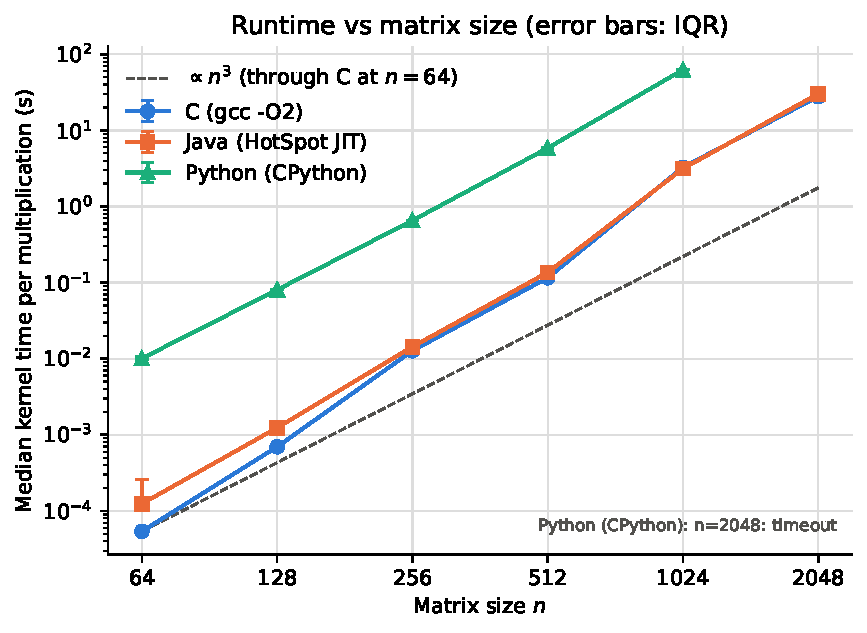
\includegraphics[width=0.78\linewidth]{fig1_time_vs_n.pdf}
  \caption{Median kernel time versus $n$ (log-log), with IQR error bars (smaller than the markers except
  for Java at $n=64$). The dashed line is a pure $n^3$ law anchored at C, $n = 64$.}
  \label{fig:time}
\end{figure}

\paragraph{Growth with $n$.} Table~\ref{tab:fit} gives the fitted slopes for $n \ge 256$. All three
are significantly above 3. The local slope between consecutive sizes, $\log_2(t(2n)/t(n))$,
shows where the excess comes from (Table~\ref{tab:local}). From 512 to 1024 the time grew by a factor of
28.3 in C and 23.1 in Java, against 8 for a cubic law. From 1024 to 2048 the growth returned to a
nearly cubic factor of 8.5 (C) and 9.6 (Java). Figure~\ref{fig:periter} shows the same effect as a step in the
time per inner-loop iteration: in C it went from 0.86\,ns at $n = 512$ to 3.05\,ns at $n = 1024$.

\begin{table}[htbp]
  \centering\small
  \caption{Least-squares fit of $\log t = a + b\log n$ on every measured repetition with $n \ge 256$.}
  \label{tab:fit}
  \begin{tabular}{llrrcr}
    \toprule
    Language & Sizes & Points & Slope $b$ & 95\% CI & $R^2$ \\
    \midrule
    C (gcc -O2)      & 256--2048 & 25 & 3.79 & [3.66, 3.92] & 0.994 \\
    Java (HotSpot)   & 256--2048 & 25 & 3.74 & [3.64, 3.84] & 0.996 \\
    Python (CPython) & 256--1024 & 20 & 3.28 & [3.25, 3.31] & 0.9996 \\
    \bottomrule
  \end{tabular}
\end{table}

\begin{table}[htbp]
  \centering\small
  \caption{Local slope $\log_2\!\big(t(2n)/t(n)\big)$ between consecutive sizes (medians); 3 corresponds
  to cubic growth.}
  \label{tab:local}
  \begin{tabular}{lccccc}
    \toprule
    Language & 64$\to$128 & 128$\to$256 & 256$\to$512 & 512$\to$1024 & 1024$\to$2048 \\
    \midrule
    C      & 3.69 & 4.19 & 3.18 & 4.82 & 3.09 \\
    Java   & 3.32 & 3.54 & 3.24 & 4.53 & 3.27 \\
    Python & 3.00 & 3.02 & 3.16 & 3.42 & -- \\
    \bottomrule
  \end{tabular}
\end{table}

\begin{figure}[htbp]
  \centering
  \begin{minipage}{0.49\linewidth}
    \centering
    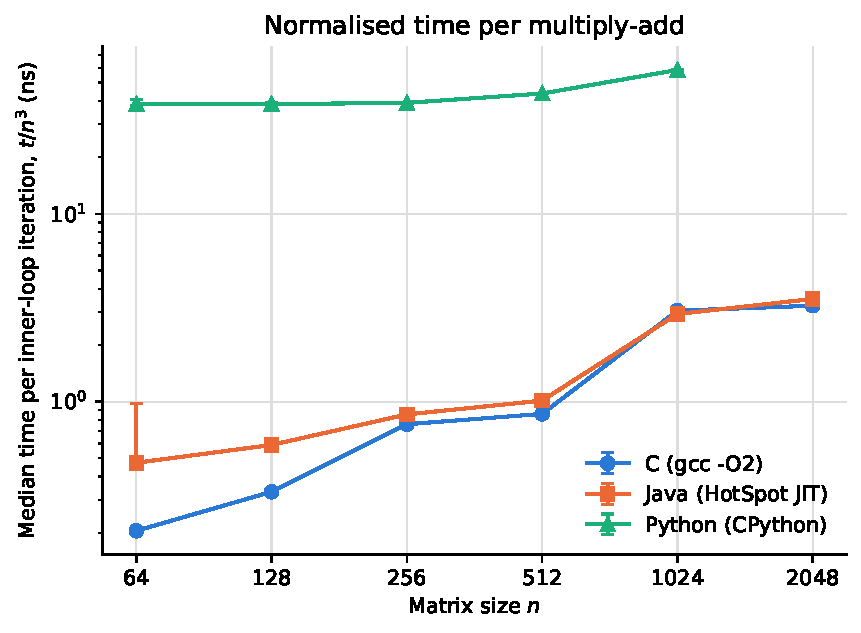
\includegraphics[width=\linewidth]{fig2_time_per_iteration.pdf}
    \caption{Median time per inner-loop iteration, $t/n^3$ (log scale).}
    \label{fig:periter}
  \end{minipage}\hfill
  \begin{minipage}{0.49\linewidth}
    \centering
    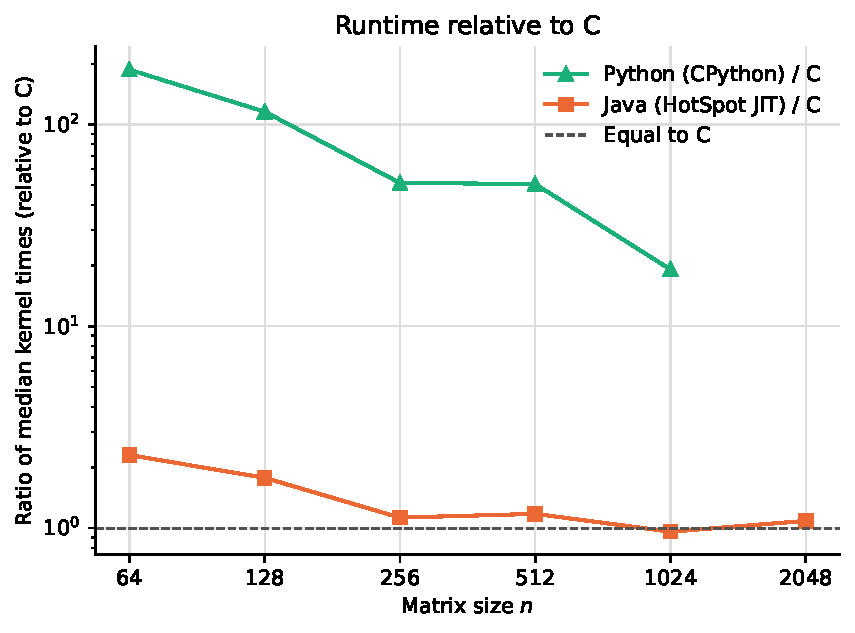
\includegraphics[width=\linewidth]{fig4_ratios.pdf}
    \caption{Ratio of median kernel times relative to C.}
    \label{fig:ratios}
  \end{minipage}
\end{figure}

\paragraph{Comparison between implementations.} Figure~\ref{fig:ratios} shows the time ratios.
CPython was 187 times slower than C at $n = 64$, about 51 times at $n = 256$ and 512, and 19 times at
$n = 1024$. Java was 2.3 times slower than C at $n = 64$ and 1.1--1.2 times slower at $n = 256$ and 512. At $n = 1024$ Java was
4\% \emph{faster} than C (3.15\,s versus 3.28\,s, with non-overlapping IQRs), and at $n = 2048$ it was
9\% slower (30.3\,s versus 27.9\,s).

\subsection{Memory}
Figure~\ref{fig:mem} plots the peak working set against the theoretical storage of the three matrices.

\begin{figure}[htbp]
  \centering
  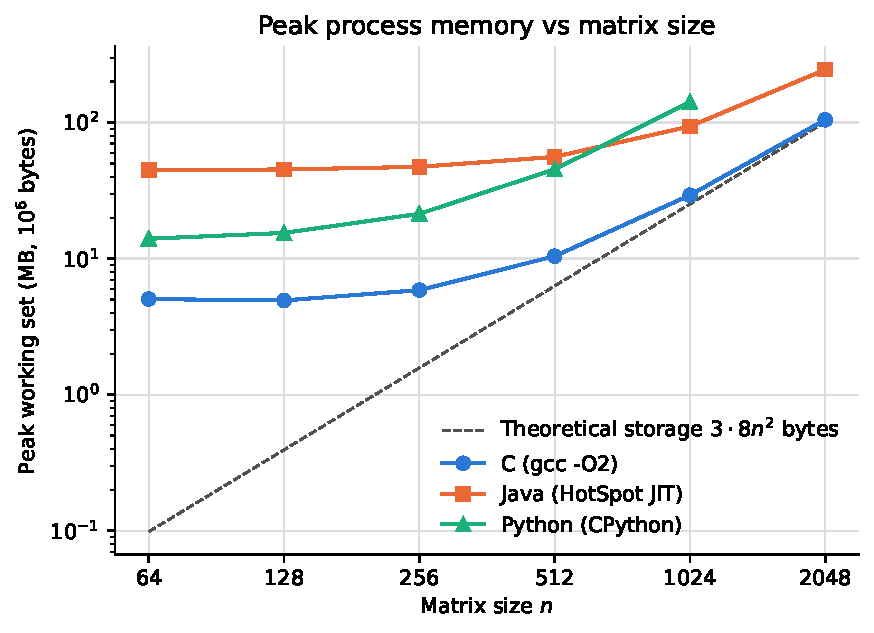
\includegraphics[width=0.72\linewidth]{fig3_peak_memory.pdf}
  \caption{Peak working set of the process (MB, $10^6$ bytes) versus $n$, and the theoretical storage of
  three dense double matrices, $24n^2$ bytes.}
  \label{fig:mem}
\end{figure}

\begin{itemize}
  \item \textbf{C:} a baseline of about 5\,MB up to $n = 256$. From then on the curve approaches the
        theoretical line: 104.8\,MB at $n = 2048$ against 100.7\,MB of matrix data.
  \item \textbf{Java:} a nearly constant baseline of about 45\,MB up to $n = 256$, reaching 244.6\,MB at
        $n = 2048$, which is 2.4 times the matrix data.
  \item \textbf{Python:} 14\,MB at $n = 64$, rising to 141\,MB at $n = 1024$, which is 5.6 times the 25.2\,MB of
        matrix data. The timed-out $n = 2048$ run had reached 514\,MB when it was stopped.
\end{itemize}

\subsection{Limits}
Under the declared budgets (Table~\ref{tab:limits}), C and Java completed every attempted size. For
CPython the largest feasible size was $n = 1024$: its single attempt at $n = 2048$ produced no result
within 600\,s. No configuration came close to the memory budget.

\begin{table}[htbp]
  \centering\small
  \caption{Feasibility under the declared budgets (600\,s per multiplication, peak working set $\le$ 50\% of RAM).}
  \label{tab:limits}
  \begin{tabular}{lrrl}
    \toprule
    Language & Max.\ attempted $n$ & Max.\ feasible $n$ & Failures \\
    \midrule
    C (gcc -O2)      & 2048 & 2048 & none \\
    Java (HotSpot)   & 2048 & 2048 & none \\
    Python (CPython) & 2048 & 1024 & $n=2048$: timeout ($>600$\,s) \\
    \bottomrule
  \end{tabular}
\end{table}

% ===========================================================================
\section{Discussion}

\paragraph{H1, cubic growth: partly supported.} The amount of arithmetic is exactly $n^3$ by
construction, but the measured time is not a fixed constant times $n^3$. The step in $t/n^3$
between $n = 512$ and $n = 1024$ coincides with the size of $B$ crossing the L2 capacity of the core
used: $B$ occupies 2\,MB at $n = 512$, which fits in the 3\,MB L2, and 8\,MB at $n = 1024$, which does not.
Because the inner loop walks down a column of $B$ with a stride of $8n$ bytes, each access then
touches a new cache line that is no longer in L2, so the loop becomes limited by memory latency
rather than by arithmetic~\cite{drepper2007,hennessy2017}. Above that point (1024$\to$2048) the growth is again close to
cubic, as expected once every size is in the same memory-bound regime. The fitted slopes of 3.7--3.8
therefore mix two regimes and do not indicate a different algorithmic complexity. The power-of-two
sizes may add conflict misses, since column strides of 4--16\,KB map many accesses to the same cache
sets~\cite{lam1991}. This interpretation was not measured directly, because no hardware performance
counters were collected, and non-power-of-two sizes were not tested.

\paragraph{H2, ranking of implementations: partly supported.} CPython was one to two orders of
magnitude slower, as predicted. Its cost per iteration (about 38\,ns up to $n = 256$) is dominated by
interpreter work: bytecode dispatch, two list indexings, boxing of each new \texttt{float} and
reference counting. This cost barely depends on the matrix size until $n \ge 512$. As C becomes
memory-bound, its per-iteration time grows by a factor of 15 while CPython's grows only by 1.5, so the Python/C
ratio shrinks from 187 to 19. The ratio therefore depends strongly on $n$, and a single ``Python is
$X$ times slower'' figure would be misleading. Java was slower than C at small $n$. At $n = 64$ a whole
multiplication takes only 0.1\,ms, so two warm-up runs are not enough for the tiered JIT to finish
optimising the kernel. Its large IQR and 3\,ms outlier point to compilation or on-stack
replacement happening during the measured repetitions; the JIT threads share the single pinned
CPU with the kernel. For $n \ge 1024$ C and Java were within $\pm$10\% of each other in both
directions, which is expected when both wait on the same memory accesses. The small Java advantage at
$n = 1024$ was reproducible within the run, but its cause (differences in the generated machine
code) was not investigated, so it should not be generalised.

\paragraph{H3, memory: supported.} At small $n$ the runtimes dominate: about 5\,MB for the C runtime,
about 45\,MB for the JVM and about 14\,MB for the CPython interpreter. At large $n$ C converges to the raw
data size. The Java excess at $n = 2048$ (about 140\,MB above the matrix data) is consistent with the
JVM baseline plus the temporary \texttt{byte[]} buffers used to read each 33.6\,MB input file
(\texttt{Files.readAllBytes}). These buffers become garbage but are still resident in the G1 heap
when the peak is taken. CPython stores each element as an 8-byte pointer to a separate 24-byte
\texttt{float} object, about 32 bytes per element instead of 8. This alone accounts for about
100\,MB at $n = 1024$, and the interpreter and temporary read buffers explain the rest of the
141\,MB observed. The scattered \texttt{float} objects also weaken locality, which plausibly explains why
CPython's $t/n^3$ also rises for $n \ge 512$.

\paragraph{Limitations.}
(i) A single laptop, OS and compiler setting were used. Results cannot be transferred to other hardware or to other
flags, and turbo frequency and temperature were not logged.
(ii) Peak working set is a process-level metric. It includes runtime overhead and transient buffers,
and it is sampled once per process (the peak across warm-up and measured repetitions).
(iii) The warm-up policy was the same for all languages. This keeps the protocol simple, but leaves Java at
$n \le 128$ partly unwarmed.
(iv) Only power-of-two sizes were tested and no hardware counters were collected, so the
cache explanation is plausible but not proven.
(v) Java at $n = 2048$ and Python at $n = 1024$ have only 5 repetitions, and Python at $n = 2048$ produced no
measurement at all.
(vi) All measurements come from one benchmark session (14 October 2026, 22:20--22:45).

% ===========================================================================
\section{Conclusions}
On this laptop and with these settings, the basic i-j-k multiplication behaved as an $n^3$
algorithm only within a memory regime. The step between $n = 512$ and $n = 1024$ that is consistent
with $B$ exceeding the L2 cache raised the cost per operation of C and Java by a factor of about 3--3.5, and
the fitted slopes reached 3.7--3.8. CPython was 19--187 times slower than C depending on $n$, and its
largest feasible size under a 600\,s budget was $n = 1024$. Compiled C and JIT-compiled Java performed
within 10\% of each other for $n \ge 1024$, while at small sizes Java paid for JIT warm-up. Memory use
approached $24n^2$ bytes for C, carried a 45\,MB runtime baseline plus input-reading buffers in Java,
and was about 5.6 times the raw data size in CPython because every element is a boxed object.

Some questions remain open. Hardware-counter measurements and non-power-of-two sizes would confirm or
refute the cache explanation, and a Java-specific warm-up study would clarify the small-$n$ results.
The cache-related step identified here is the natural target for the loop-reordering and blocking
optimisations of Assignment~2.

% ===========================================================================
\section*{Reproducibility materials}
All code, configuration and raw data are available at \repo{} (folder \texttt{assignment1/}). The
\texttt{README.md} gives the exact commands, all run from the repository root:
\begin{lstlisting}
pip install -r requirements.txt
python assignment1/scripts/generate_inputs.py
python assignment1/scripts/system_info.py
powershell -ExecutionPolicy Bypass -File assignment1/scripts/build.ps1
python assignment1/scripts/validate.py
python assignment1/scripts/run_benchmarks.py
python assignment1/scripts/analyze.py
\end{lstlisting}
Raw measurements: \texttt{results/raw/benchmark\_20261014\_222025.csv} (one row per warm-up and
measured repetition, never filtered) with its metadata JSON; validation:
\texttt{results/validation.csv}; environment: \texttt{results/system\_info.json};
session notes: \texttt{results/run\_notes.md}; tables and figures: \texttt{results/tables/},
\texttt{figures/}.

\section*{Use of generative AI}
Claude (Anthropic) was used through the Claude app and Claude Code for: planning the experimental
protocol, generating and debugging the kernels and scripts (input generation, validation,
benchmark orchestration, analysis and plotting), and drafting and language revision of this report.
The author reviewed the code, ran all builds, tests and benchmarks on his own laptop, and checked
that every number in this report matches the raw CSV and the generated tables. No measurement or reference was
produced by the AI tool without being checked against the data or the cited source.

% ===========================================================================
\begin{thebibliography}{9}

\bibitem{golub2013}
G.~H. Golub and C.~F. Van~Loan, \emph{Matrix Computations}, 4th~ed.
Baltimore, MD, USA: Johns Hopkins Univ. Press, 2013.

\bibitem{higham2002}
N.~J. Higham, \emph{Accuracy and Stability of Numerical Algorithms}, 2nd~ed.
Philadelphia, PA, USA: SIAM, 2002.

\bibitem{drepper2007}
U.~Drepper, ``What every programmer should know about memory,'' Red Hat, Inc., Tech. Rep., Nov. 2007.
[Online]. Available: \url{https://people.freebsd.org/~lstewart/articles/cpumemory.pdf}

\bibitem{hennessy2017}
J.~L. Hennessy and D.~A. Patterson, \emph{Computer Architecture: A Quantitative Approach}, 6th~ed.
Cambridge, MA, USA: Morgan Kaufmann, 2017.

\bibitem{lam1991}
M.~D. Lam, E.~E. Rothberg, and M.~E. Wolf, ``The cache performance and optimizations of blocked
algorithms,'' in \emph{Proc. 4th Int. Conf. Architectural Support for Programming Languages and
Operating Systems (ASPLOS IV)}, 1991, pp.~63--74.

\bibitem{georges2007}
A.~Georges, D.~Buytaert, and L.~Eeckhout, ``Statistically rigorous Java performance evaluation,''
in \emph{Proc. 22nd ACM SIGPLAN Conf. Object-Oriented Programming Systems, Languages and Applications
(OOPSLA)}, 2007, pp.~57--76.

\bibitem{ms_pmc}
Microsoft, ``PROCESS\_MEMORY\_COUNTERS structure (psapi.h),'' Win32 API documentation.
[Online]. Available: \url{https://learn.microsoft.com/en-us/windows/win32/api/psapi/ns-psapi-process_memory_counters}

\bibitem{ms_cpuset}
Microsoft, ``GetSystemCpuSetInformation function (processthreadsapi.h),'' Win32 API documentation.
[Online]. Available: \url{https://learn.microsoft.com/en-us/windows/win32/api/processthreadsapi/nf-processthreadsapi-getsystemcpusetinformation}

\bibitem{ms_qpc}
Microsoft, ``Acquiring high-resolution time stamps,'' Win32 documentation.
[Online]. Available: \url{https://learn.microsoft.com/en-us/windows/win32/sysinfo/acquiring-high-resolution-time-stamps}

\end{thebibliography}

\end{document}
